\documentclass[14pt]{extreport}

% Основные пакеты
\usepackage[english, russian]{babel}    % Поддержка русского и английского языков
\usepackage{graphicx}                   % Для вставки изображений
\usepackage{import}                     % Для продвинутого импорта (например, pdf_tex из Inkscape)
\usepackage{subcaption}                 % Для создания подписей к фигурам
\usepackage{float}                      % Для улучшенного позиционирования фигур
\usepackage{geometry}                   % Для управления отступами на странице
\usepackage{amsmath}                    % Для расширенной поддержки математики
\usepackage{amsfonts}                   % Математические шрифты
\usepackage{amssymb}                    % Математические символы
\usepackage{tabu}                       % Улучшенные таблицы
\usepackage{booktabs}                   % Профессиональные таблицы с вертикальными разделителями
\usepackage[dvipsnames]{xcolor}         % Расширенная поддержка цветов
\usepackage{longtable}                  % Для таблиц, занимающих несколько страниц
\usepackage{makecell}                   % Для улучшенного форматирования ячеек таблиц
\usepackage{multirow}                   % Для объединения строк в таблицах
\usepackage{tabularray}                 % Для современных таблиц
\usepackage{varwidth}                   % Для переменной ширины блоков
\usepackage{hyperref}                   % Для гиперссылок
\usepackage{verbatim}                   % Для вставки кода
\usepackage{listings}                   % Для оформления листингов кода
\usepackage{amsmath}
% Настройка графики
\graphicspath{ {./images/} }            % Путь к папке с изображениями

% Настройка отступов на странице
\geometry{left=2cm, right=2cm, bottom=2cm, top=2cm}

% Настройка гиперссылок
\hypersetup{
	linkcolor=blue,                     % Цвет ссылок
	filecolor=magenta,                  % Цвет ссылок на файлы
	urlcolor=cyan                       % Цвет URL-адресов
}

\definecolor{codegreen}{rgb}{0,0.6,0}  % Цвет для комментариев
\definecolor{codegray}{rgb}{0.5,0.5,0.5}  % Цвет для номеров строк
\definecolor{codepurple}{rgb}{0.58,0,0.82}  % Цвет для строк
\definecolor{backcolour}{rgb}{0.95,0.95,0.92}  % Цвет фона

% Определим стиль для выделения переменных
\lstdefinestyle{codestyle}{
	backgroundcolor=\color{backcolour},  % Цвет фона
	commentstyle=\color{codegreen}\itshape,  % Стиль для комментариев
	keywordstyle=\color{magenta}\bfseries,  % Стиль для ключевых слов
	numberstyle=\tiny\color{codegray},  % Стиль для номеров строк
	stringstyle=\color{codepurple},  % Стиль для строк
	identifierstyle=\color{black},  % Стиль для переменных (выделим их синим)
	basicstyle=\ttfamily\footnotesize,  % Размер шрифта для кода
	breakatwhitespace=false,  % Не разрывать строки в пробелах
	breaklines=true,  % Разбивать длинные строки
	captionpos=b,  % Позиция заголовка (внизу)
	keepspaces=true,  % Сохранять пробелы
	numbers=left,  % Позиция номеров строк
	numbersep=10pt,  % Расстояние между кодом и номерами строк
	showspaces=false,  % Не показывать пробелы
	showstringspaces=false,  % Не показывать пробелы в строках
	showtabs=false,  % Не показывать табуляции
	tabsize=4,  % Размер табуляции
	frame=single,  % Добавить рамку вокруг кода
	rulecolor=\color{black},  % Цвет рамки
	backgroundcolor=\color{backcolour},  % Цвет фона рамки
	xleftmargin=15pt,  % Отступ слева
	xrightmargin=15pt,  % Отступ справа
}


\lstset{style=codestyle}
\lstset{extendedchars=\true}
\graphicspath{{../images/}}

\begin{document}
	
	\begin{titlepage}
		\centering
		\vspace*{1cm}
		
		{\large Министерство науки и высшего образования Российской Федерации}\\
		{\large ФЕДЕРАЛЬНОЕ ГОСУДАРСТВЕННОЕ АВТОНОМНОЕ ОБРАЗОВАТЕЛЬНОЕ УЧРЕЖДЕНИЕ ВЫСШЕГО ОБРАЗОВАНИЯ «НАЦИОНАЛЬНЫЙ ИССЛЕДОВАТЕЛЬСКИЙ УНИВЕРСИТЕТ ИТМО»}\\
		{\large (УНИВЕРСИТЕТ ИТМО)}\\
		
		\vspace{1cm}
		
		\textbf{{\Huge ОТЧЕТ}\\
			{\Huge ПО ЛАБОРАТОРНОЙ РАБОТЕ №4}}\\
		
		\vspace{1cm}
		
		{\LARGE По дисциплине\\
			\(\lll\) Математическая Статистика \(\ggg\) }\\
			Вариант 2
		
		\vspace{2cm}
		
		{\Large Студенты:}\\
		Охрименко Eва\\
		Даниил Буцкий
		
		
		\vspace{2cm}
		
		{\Large Проверил:}\\
		Шкваренко Андрей Алексеевич\\
		
		\vspace{2cm}
		
		{\large г. Санкт-Петербург}\\
		{\large 2025}
		
	\end{titlepage}
	\tableofcontents  % Оглавление
	\newpage

	
	
	\section{Вопрос}
	
	
	В этом задании нужно оценить однородность количества мужчин и жещин в эксперименте. Также нужно оценить этническую принадлежность. Вот код, который считает данные полов и данные этнических принадлежностей из файла:
	
	
	\begin{lstlisting}[language=python, caption={Счет данных по выборкам}]
f = open('exams_dataset.csv')

maleCount = femaleCount = 0
countA = countB = countC = countD = countE = 0

for line in f:
	
	items = line.strip().replace('"', '').split(',')
	
	gender = items[0]
	etnic = items[1]
	
	if gender == 'male':
	maleCount += 1
	elif gender == 'female':
	femaleCount += 1
	
	if etnic[-1] == 'A':
	countA += 1
	elif etnic[-1] == 'B':
	countB += 1
	elif etnic[-1] == 'C':
	countC += 1
	elif etnic[-1] == 'D':
	countD += 1
	elif etnic[-1] == 'E':
	countE += 1


genderArray = list()
etnicArray = list()

genderArray += [maleCount, femaleCount]
etnicArray += [countA, countB,  countC,  countD, countE]
\end{lstlisting}
	
	
	У нас получилось \texttt{506} мужчин и \texttt{494} женщин. Также у нас получился такой массив по этническим группам: \texttt{[77, 204, 324, 261, 134]}. Можно заметить, что массив с полами примерно однороден, а с этническими группами менее однороден.
	
	\subsection{Реализация методов}	
	
	Для этого задания мы напишем 2 статистических метода на питоне. Метод \texttt{хи-квадрат} и метод вычисляющдий \texttt{критерий Когломорова-Смирнова}
	
	Итак, критерий \texttt{хи-квадрат} вычисляется по формуле:
	
	\[
		\chi^2 = \sum_{i=1}^{n} \frac{(O_i - E_i)^2}{E_i}
	\]
	
	где:
	\begin{itemize}
		\item $O_i$ --- наблюдаемые значения (элементы массива \texttt{array})
		\item $E_i = \frac{\sum_{j=1}^{n} O_j}{n}$ --- ожидаемое значение для равномерного распределения
		\item $n$ --- количество элементов в массиве (\texttt{ln = len(array)})
	\end{itemize}
	
	А \texttt{критерий Когломорова-Смирнова} вычисляется так:
	
	\[
		D_n = \sup_x |F_n(x) - F(x)|
	\] 
	
	где:
	\begin{itemize}
		\item $F_n(x)$ --- эмпирическая функция распределения:
		\[
			F_n(x) = \frac{\text{количество элементов} \leq x}{n} = \frac{i}{n} \quad \text{для} \quad x \in [x_{(i)}, x_{(i+1)})
		\] 
		
		\item $F(x)$ --- теоретическая функция равномерного распределения:
		\[
			F(x) = \frac{x}{\max(\text{array})} \quad \text{для} \quad x \in [0, \max(\text{array})]
		\] 
		
		\item $\sup_x$ --- супремум (максимальное отклонение)
	\end{itemize}
	
	Вот реализация кодом:
	
	\begin{lstlisting}[language=python, caption=Расчет хи-квадрат]
def hiQuad(array):
	
	sm = sum(array)
	ln = len(array)
	expected = sm / ln
	
	hiQuad = sum((i - expected)**2 / expected for i in array)   
	
	return round(hiQuad, 4)
\end{lstlisting}
	
	\begin{lstlisting}[language=python, caption=Расчет критерия Когломорова-Смирнова]
def kolmogorovSmirnov(array):
	
	ln = len(array)
	sortArray = np.sort(array)
	
	y = np.arange(1, ln+1) / ln
	teoria = sortArray / np.max(sortArray)
	kriteriy = np.max(np.abs(y - teoria))
	
	return round(kriteriy, 4)
\end{lstlisting}
	
	\subsection{Применение методов к выборкам}
	
	Применяем методы:
	
	\begin{lstlisting}[language=python, caption=Применение метода к гендерам]
result = hiQuad(genderArray)
print(result)

Output >>> 0.144
\end{lstlisting}
	
	
	\begin{lstlisting}[language=python, caption=Применение метода к этникам]
result = kolmogorovSmirnov(etnicArray)
print(result)

Output >>> 0.0377
\end{lstlisting}
	
	\subsection{Оценка и вывод}
	
	
	Для начала сформулируем гипотезы для полов:
	
	\begin{itemize}
		\item \texttt{Нулевая гипотеза:} Распределение полов равномерное (50 на 50)
		\item \texttt{Альтернативная гипотеза:} Распределение полов неравномерное
	\end{itemize}

	Теперь посчитаем критическое значение хи квадрат по таблице из интернета
	
	\begin{figure}[H]
		\centering
		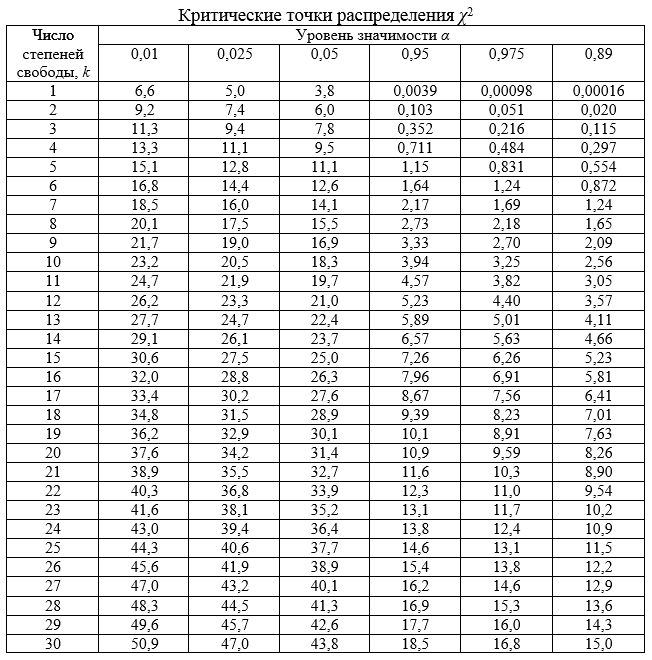
\includegraphics[width=1\textwidth]{table.png}
		\caption{Таблица}
		\label{fig:lines}
	\end{figure}
	
	Нам нужно взять $k = 1$, так как оно считается по формуле $k = iterations - 1$ (посчитали по туториалу)и возьмем $\alpha = 0.05$ - средний уровень значимости
	
	Тогда наше критическое значение $\chi_{crit}^2 = 3.8$. Так как $\chi_{crit}^2 > \chi^2$, то вывод таков: \texttt{распредедление полов равномерное}.
	
	Теперь сформулируем гипотезы для этнических принадлежностей:
	
	\begin{itemize}
		\item \texttt{Нулевая гипотеза:} Распределение этник равномерное 
		\item \texttt{Альтернативная гипотеза:} Распределение этник неравномерное
	\end{itemize}
	
	
	
\end{document}